\makeatletter
\def\input@path{{../}}
\makeatother
\documentclass[../main.tex]{subfiles}

\begin{document}

\chapter{Теория групп}
\section{Группы и подгруппы, новые примеры}%

\rmk{Примеры.}

\textbf{\rom{1}}.\, Аддитивные подгруппы следующих колец: $\Z,\, \Q,\, \R,\, \C$, кольцо многочленов $A[x]$, поле дробно-рациональных функций $K(x)$, кольцо квадратных матриц $M(n, A)$. Аддитивная группа кольца обычно обозначается так же, как и само кольцо. То есть группа $\Z$ обозначает группу $(\Z, +)$, группа $\Q$ обозначает группу $(\Q, +)$ и так далее.

\begin{remark}
    Запись $A < B$ означает, что $A$ является подгруппой группы $B$.
\end{remark}

 Зафиксируем некоторое целое число $m \in \Z$. Введем отношение "быть сравнимым по модулю $m$" на множестве целых чисел(обозначение $\overset{m}{\equiv}$).

\begin{equation*}
    a \overset{m}{\equiv} b \iff a - b \, \vdots \, m
\end{equation*}

\begin{statement}
    $\overset{m}{\equiv}$ - отношение эквивалентности на $\Z$.
\end{statement}

Фактор-множество по отношению сравнимости по модулю $m$ обозначается как $\Z/m\Z$ или $\Z/(m)$.

\begin{statement}
Это множество состоит ровно из $m$ элементов(классов).
\begin{equation*}
    \Z/_{\overset{m}{\equiv}} = \Z/m\Z = \Z/(m) \underset{m > 0}{=} \{[0], [1], \dotsc, [m - 1]\}
\end{equation*}
\end{statement}
\begin{proof}
    Классов будет не больше чем $m$, потому что у каждого числа есть остаток при делении на $m$. То есть:
    \begin{equation*}
        a = mq + r \implies a \equiv r \pmod m \implies a \in [r]
    \end{equation*}
    $r$ пробегает по всем остаткам $m$, значит $r$ может принимать всего $m$ различных значений. При этом, все остатки образуют различные классы. В противном случае:
    \begin{equation*}
        \begin{cases*}
            0 \leq k < l \leq m - 1 \implies (l - k) \in (0, m - 1] \\
            [k] = [l]  \implies l - k\, \vdots\, m
        \end{cases*}
    \end{equation*}
    Противоречие. Значит у нас $m$ различных классов, что и требовалось доказать.
\end{proof}

Введем на $\Z/m\Z$ сложение и умножение:

\begin{center}
\begin{tabular}{l p{2.5cm} r}
    $[a] + [b ] \coloneqq [a + b]$ &  & $[a] \cdot [b] \coloneqq [a \cdot b]$
\end{tabular}
\end{center}

Проверка корректности заданных операций была в курсе дискретной математики.
\begin{theorem-non}
    $(\Z/m\Z, +, \cdot)$ - коммутативное, ассоциативное кольцо с единицей.
\end{theorem-non}
\begin{definition}
    $(\Z/m\Z, +, \cdot)$ называется \textbf{кольцом класса вычетов по модулю $m$}.
\end{definition}

\rmk{Обобщения.}

\textbf{1}. Конструкцию построения кольца класса вычетом можно обобщить на произвольное коммутативное кольцо $R$. Возьмем произвольный элемент $f \in R$ и рассмотрим отношение сравнимости по модулю этого элемента {\scriptsize${\overset{f}{\equiv}}$}. Дальше можно перейти к множеству классов эквивалентности по данному отношению $R/(f) = R/_{\overset{f}{\equiv}}$. Можно показать, что получившаяся структура является факторкольцом. В частности, если взять в качестве исходного кольца кольцо многочленов над $R$, то верно следующее равенство:
\begin{equation*}
    \R[x]/_{(x^2 + 1)} = \C
\end{equation*}
Читателю предлагается доказать этот факт самостоятельно.
\pagebreak

\textbf{2}. Так же можно ввести понятие \textit{сравнимости по модулю идеала $I$} на коммутативном кольце $R$.
\begin{equation*}
    a \overset{I}{\equiv} b \iff a - b \in I
\end{equation*}
Аналогичным образом определяется кольцо классов вычетов $R/_I = R/_{{\overset{I}{\equiv}}}$

\textbf{\rom{2}}. Пусть $A$ - ассоциативное коммутативное кольцо с единицей. Тогда множество
обратимых элементов \linebreak $A^{*} = \{a \in A \, | \, \exists \, b \in A \, : \, ab = ba =
1\}$ образует группу по умножению. В частности $\Z^{*}, \Q^{*}, \R^{*}, \C^{*}$ являются
мультипликативными группами. Еще один интересный пример --- множество обратимых матриц $M(n, K)^{*
} = \GL(n, K)$. Такое множество называется \textit{общей линейной группой} степени $n$ над полем
$K$. Важная подгруппа $\GL(n, K)$ --- множество $\SL(n, K) = \{A \in \GL(n, K) \, | \, |A| = 1\}$
называемое \textit{специальной линейной группой}, состоит из обратимых матриц, с определителем
равным единице. Множество скалярных матриц над кольцом также является мультипликативной группой.
Напомним, что скалярной матрицей называется диагональная матрица, элементы главной диагонали
которой равны.

Еще одним важным примером является множество обратимых элементов в кольце вычетов по модулю $m$. Заметим, что $(\Z/m\Z)^{*} = \{[a] \, | \, (a, m) = 1\}$. Также очевидно, что $|(\Z/m\Z)^{*}| = \varphi(m)$, где $\varphi(m)$ --- это функция Эйлера от числа $m$.

\rmk{Факт}. Группа $\Z/m\Z$ является циклической, потому что $\Z/m\Z = \langle[1]\rangle$. При этом группа обратимых по умножению элементов может как быть, так и не быть циклической. Например, $(\Z/5\Z)^{*} = \langle[2]\rangle$, при этом легко показать, что $(\Z/8\Z)^{*}$ не порождается ни одним из своих элементов.

\begin{exercise}
    При каких $m$ группа(относительно умножения) $(\Z/m\Z)^{*}$ является циклической?
\end{exercise}

\textbf{\rom{3}}. $S_n = S(\{1, 2, \dotsc, n\})$ --- группа перестановок чисел от $1$ до $n$. $A_n = \{\sigma \in S_n \, | \, \sgn \sigma = 1\}$ --- множество четных перестановок является подгруппой $S_n$ относительно операции композиция.

\textbf{\rom{4}}. Пусть $\Phi$ --- фигура на плоскости, $\Sigma(\Phi)$ --- самосовмещения $\Phi$. $D_n$ --- группа симметрий правильного $n$-угольника(группа диэдра).

\begin{center}
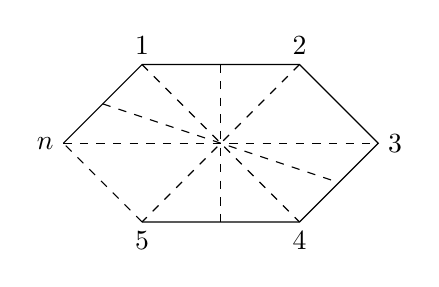
\begin{tikzpicture}
\draw[-] (0, 0) -- (1, 1) -- (3, 1) -- (4, 0) -- (3, -1) -- (1, -1);
\draw[dashed, -] (1, -1) -- (0, 0);
\draw[dashed, -] (0, 0) -- (4, 0);
\draw[dashed, -] (1, 1) -- (3, -1);
\draw[dashed, -] (3, 1) -- (1, -1);
\draw[dashed, -] (2, 1) -- (2, -1);
\draw[dashed, -] (0.5, 0.5) -- (3.5, -0.5);
\fill (0,0) node[left] {$n$};
\fill (1,1) node[above] {1};
\fill (3,1) node[above] {2};
\fill (4,0) node[right] {3};
\fill (3,-1) node[below] {4};
\fill (1,-1) node[below] {5};
\end{tikzpicture}
\end{center}
Легко видеть, что повороты $R_n$ $n$-угольника на углы, кратные $\frac{2\pi}{n}$(то есть углы вида $k \cdot \frac{2\pi}{n}, k = 0, 1, \dotsc, n - 1$) являются самосовмещениями. Так же есть $n$ симметрий $S_k, k = 0, 1, \dotsc, n - 1$. В случае нечетного $n$ все оси симметрии будут проходить через вершины, в случае четного $n$ половина осей симметрии будет проходить через середины сторон. Таким образом $D_n$ --- группа порядка $2n$.
\begin{exercise}
    Построить таблицу Кэли для группы $D_n$(содержательная часть задачи --- понять что такое умножение поворота на симметрию, симметрии на поворот, симметрии на симметрию и поворота на поворот).
\end{exercise}

Еще несколько интересных примеров групп. Множество обратимых комплексных чисел, с модулем равным единице $\mathbb{T} = \{z \in \C^{*} \, | \, |z| = 1\}$ явлется мультипликативной подгруппой $\C^{*}$. Также внутри $\mathbb{T}$ есть $\mu_n = \{z \in \C \, | \, z^n = 1\}$ --- множество всех корней $n$-ной степени из единицы. Оказывается, что $\mu_n$ является мультипликативной циклической(порождается, например, элементом $\zeta_1$) подгруппой $\C$.

\section{Подгруппа, порождённая подмножеством}

Пусть $G$ --- группа, $g \in G$ --- элемент в этой группе. Тогда $\langle g \rangle$ обозначает множество всех степеней элемента $g$. То есть $\langle g \rangle = \{g^n \, | \, n \in \Z\}$.
\begin{statement}
    $\langle g \rangle$ --- группа.
\end{statement}
\begin{proof}
    1. $g^m \cdot g^n = g^{m + n}$ --- замкнутость, относительно умножения.

    2. $(g^m)^{-1} = g^{-m}$ --- замкнутость, относительно взятия обратного.

    3. $e = g^{0}$ --- нейтральный принадлежит подгруппе.
\end{proof}
$\langle g \rangle$ также называют \textit{циклической подгруппой, порожденной $g$}.
\begin{definition}
    Группа называется \textbf{циклической}, если существует элемент, который её порождает.
\end{definition}
\begin{definition}
    \textbf{Порядок элемента} $g$ --- минимальное натуральное число $n$, такое что $g^n = e$. Если такого числа нет, то порядок считается равным бесконечности. Формально:
    \begin{align*}
        &\ord g = \min \{n \in \N \, | \, g^n = e\}\\
        &\ord g = +\infty\text{, если таких $n$ нет}
    \end{align*}
\end{definition}
\begin{theorem-non}
    1. $|\langle g \rangle| = \ord g$

    2. $\ord g = n < +\infty \implies \langle g \rangle = \{g^{0}, g^{1}, \dotsc, g^{n - 1}\}$
\end{theorem-non}
\begin{proof}
    \rom{1}. Пусть $\ord g = +\infty$. Пусть $i, j \in \Z, 0 < i < j$. Тогда:
    \begin{equation*}
        g^{j - i} \neq e \implies g^{j} \neq g^{i}
    \end{equation*}
    То есть любые две степени элемента $g$ не равны между собой. Значит $|\langle g \rangle| = +\infty$.

    \rom{2}. Пусть $\ord g = n < +\infty$. Тогда $m = nq + r, \, 0 \leq r \leq n - 1$. Отсюда:
    \begin{equation*}
        g^m = (g^n)^{q} \cdot g^r = (e)^{q} \cdot g^r = g^r \implies \langle g \rangle = \{g^0, g^1, \dotsc, g^{n - 1}\}
    \end{equation*}
    Для первого утверждения осталось показать, что $|\{g^0, g^1, \dotsc, g^{n - 1}\}| = n$, то есть $g^i \ne g^j, \, 0 \leq i < j \leq n - 1$:
    \begin{equation*}
    \begin{gathered}
        \ord g = n \implies g^x \neq e, \forall x \in [1, n - 1]  \implies g^{j - i} \neq e,\forall (j - i) \in [1, n - 1] \\
        \implies g^{j} \neq g^{i}, \forall i,j \in \Z, 0 \leq i < j \leq n - 1
    \end{gathered}
    \end{equation*}
    Что и требовалось доказать.
\end{proof}
\begin{remark}
    1. $\ord g = +\infty \implies \langle g \rangle \cong \Z$

    2. $\ord g = n \implies \langle g \rangle \cong \Z/n\Z$

    \textit{(от редакторов конспекта)} Действительно, легко видеть, что отображение $a \mapsto g^a$ является изоморфизмом.
\end{remark}
\begin{definition}
    Пусть $G$ - группа, $M \subset G$. Тогда:

    $\langle M \rangle = \{g_1 \dotsm g_s \, | \, s \geq 0,\, g_1, \dotsc, g_s \in M \cup M^{-1}\}$ --- \textbf{подгруппа, порожденная $M$}.
\end{definition}
\begin{remark}
    $\langle \{g\} \rangle = \langle g \rangle$
\end{remark}
\begin{theorem-non}
    $\langle M \rangle$ - подгруппа $G$.
\end{theorem-non}
\begin{proof}
    1. Нейтральный элемент очевидно попал в $\langle M \rangle$ как произведение нуля сомножителей.

    2. $(g_1 \dotsm g_s) \cdot (g_1' \dotsm g_t') = g_1 \dotsm g_s g_1' \dotsm g_t' \in \langle M \rangle$ - замкнутость относительно умножения.

    3. $(g_1 \dotsm g_s)^{-1} = g_s^{-1} \dotsm g_1^{-1} \in \langle M \rangle$ - замкнутость относительно взятия обратного.
\end{proof}
\begin{remark}
    Объединение подгрупп - подгруппа. Формально:
    \begin{equation*}
        H_i < G, \, i \in I \implies \bigcap_{i \in I} H_i < G
    \end{equation*}
\end{remark}
\begin{theorem-non}
    \begin{equation*}
        \langle M \rangle = \bigcap_{\substack{H < G \\ M \subset H}} H
    \end{equation*}
\end{theorem-non}
\begin{proof}
    1. $\encircle{\bigsubset[1.5]}$ Надо показать, что если $H < G$ и $M \subset H$, то $\langle M \rangle \subset H$:
    \begin{equation*}
        M \subset H \underset{\mathclap{\text{замкнутость относительно взятия обратного}}}{\implies} M^{-1} \subset H \implies g_1, \dotsc, g_s \in H (g_i \in M \cup M^{-1}) \underset{\mathclap{\text{замкнутость относительно умножения}}}{\implies} \langle M \rangle \subset H
    \end{equation*}

    2. $\encircle{\bigsupset[1.5]}$ Заметим, что среди $H$ найдется и $\langle M \rangle$, потому что $\langle M \rangle < G$, а также $M \subset \langle M \rangle$. А так как пересечение $\langle M \rangle$ с какими-то другими множествами точно будет не больше чем $\langle M \rangle$, то $\langle M \rangle M \supset \bigcap H$.
\end{proof}
Вместо $\langle \{g_1, \dotsc, g_t\} \rangle$ обычно пишут $\langle g_1, \dotsc, g_t \rangle$.
\begin{remark}
    $S_n = \langle (1 2 \dotso n), (1 2)\rangle = \langle (2 \dotso n), (1 2) \rangle$; \quad $D_n = \langle R_1, S_\sigma \rangle$
\end{remark}
\begin{exercise}
    Придумать пример конечной группы, не порождаемой двумя элементами.
\end{exercise}

\section{Гомоморфизмы}
\begin{definition}
    Отображение $G \overset{\varphi}{\to} G'$($G, G'$ --- группы) называется \textbf{гомоморфизмом групп}, если
\begin{equation*}
    \forall g_1, g_2 \in G\colon \varphi(g_1g_2) = \varphi(g_1)\varphi(g_2)
\end{equation*}
\end{definition}
\rmk{Примеры.}

1. $\R \to C^{*}$, $\alpha \mapsto \cos \alpha + i \sin \alpha$

2. $G$ - абелева группа, $m \in \Z$

$G \to G$, $g \mapsto g^m$

3. $S_n \to \Z^{*}$, $\sigma \mapsto \sgn \sigma$

\begin{definition}
    Пусть $\varphi$ --- гомоморфизм. Тогда:

    \begin{equation*}
        \begin{gathered}
            \Im \varphi = \{\varphi(g) \, | \, g \in G\}\text{ --- \textbf{ядро гомоморфизма}}\\
            \Ker \varphi = \{g \in G \, | \, \varphi(g) = e\}\text{ --- \textbf{образ гомоморфизма}}
        \end{gathered}
    \end{equation*}
\end{definition}

\begin{theorem-non}
    Пусть $\varphi\colon G \to G'$ --- гомоморфизм. Тогда $\Im \varphi$ --- подгруппа $G'$, а $\Ker \varphi$ --- подгруппа $G$.
\end{theorem-non}
\begin{proof}
    Сначала докажем лемму.
    \begin{lemma}
    \label{lem:6.1}
        Образ нейтрального элемента --- нейтральный элемент. Формально:
        \begin{equation*}
            \varphi(e_{G}) = e_{G'}
        \end{equation*}
    \end{lemma}
    \begin{proof}
        \begin{equation*}
            \begin{gathered}
                e_G \cdot e_G = e_G \\
                \varphi(e_G) \cancel{\varphi(e_G)} = \cancel{\varphi(e_G)}\\
                \varphi(e_G) = e_{G'}
            \end{gathered}
        \end{equation*}
        Лемма доказана.
    \end{proof}
    Сначала докажем утверждение для образа.
    \begin{equation*}
        \begin{gathered}
            \varphi(g_1) \varphi(g_2) = \varphi(g_1g_2) \in \Im \varphi \text{ --- замкнутость относительно умножения}\\
            \varphi(g) \varphi(g^{-1}) = \varphi(g g^{-1}) = \varphi(e_G) \underset{\mathclap{\text{по лемме \ref{lem:6.1}}}}{=} e_{G'} \implies \varphi^{-1}(g) = \varphi(g^{-1}) \in \Im \varphi \text{ --- замкнутость относительно взятия обратного}\\
            e_{G'} \underset{\mathclap{\text{по лемме \ref{lem:6.1}}}}{=} \varphi(e_G) \in \Im \varphi \text{ --- нейтральный попадает в образ}
        \end{gathered}
    \end{equation*}
    Таким образом $\Im \varphi < G'$. Теперь докажем утверждение для ядра.
    \begin{equation*}
        \begin{gathered}
            \varphi(e_G) = e_{G'}\text{ --- нейтральный $e_G$ попадает в ядро} \\
            \varphi(g_1g_2) = \varphi(g_1)\varphi(g_2) = e_{G'}e_{G'} = e_{G'}\text{ --- замкнутость относительно умножения}\\
            \varphi(g^{-1}) = \varphi(g)^{-1} = (e_{G'})^{-1} = e_{G'}\text{ --- замкнутость относительно взятия обратного}
        \end{gathered}
    \end{equation*}
    Значит $\Ker \varphi < G$. Предложение доказано.
\end{proof}
\end{document}
